% Options for packages loaded elsewhere
\PassOptionsToPackage{unicode}{hyperref}
\PassOptionsToPackage{hyphens}{url}
\PassOptionsToPackage{dvipsnames,svgnames,x11names}{xcolor}
%
\documentclass[
  11pt,
  a4paper,
]{article}
\usepackage{amsmath,amssymb}
\usepackage{iftex}
\ifPDFTeX
  \usepackage[T1]{fontenc}
  \usepackage[utf8]{inputenc}
  \usepackage{textcomp} % provide euro and other symbols
\else % if luatex or xetex
  \usepackage{unicode-math} % this also loads fontspec
  \defaultfontfeatures{Scale=MatchLowercase}
  \defaultfontfeatures[\rmfamily]{Ligatures=TeX,Scale=1}
\fi
\usepackage{lmodern}
\ifPDFTeX\else
  % xetex/luatex font selection
\fi
% Use upquote if available, for straight quotes in verbatim environments
\IfFileExists{upquote.sty}{\usepackage{upquote}}{}
\IfFileExists{microtype.sty}{% use microtype if available
  \usepackage[]{microtype}
  \UseMicrotypeSet[protrusion]{basicmath} % disable protrusion for tt fonts
}{}
\makeatletter
\@ifundefined{KOMAClassName}{% if non-KOMA class
  \IfFileExists{parskip.sty}{%
    \usepackage{parskip}
  }{% else
    \setlength{\parindent}{0pt}
    \setlength{\parskip}{6pt plus 2pt minus 1pt}}
}{% if KOMA class
  \KOMAoptions{parskip=half}}
\makeatother
\usepackage{xcolor}
\usepackage[margin=0.85in]{geometry}
\usepackage{longtable,booktabs,array}
\usepackage{calc} % for calculating minipage widths
% Correct order of tables after \paragraph or \subparagraph
\usepackage{etoolbox}
\makeatletter
\patchcmd\longtable{\par}{\if@noskipsec\mbox{}\fi\par}{}{}
\makeatother
% Allow footnotes in longtable head/foot
\IfFileExists{footnotehyper.sty}{\usepackage{footnotehyper}}{\usepackage{footnote}}
\makesavenoteenv{longtable}
\usepackage{graphicx}
\makeatletter
\def\maxwidth{\ifdim\Gin@nat@width>\linewidth\linewidth\else\Gin@nat@width\fi}
\def\maxheight{\ifdim\Gin@nat@height>\textheight\textheight\else\Gin@nat@height\fi}
\makeatother
% Scale images if necessary, so that they will not overflow the page
% margins by default, and it is still possible to overwrite the defaults
% using explicit options in \includegraphics[width, height, ...]{}
\setkeys{Gin}{width=\maxwidth,height=\maxheight,keepaspectratio}
% Set default figure placement to htbp
\makeatletter
\def\fps@figure{htbp}
\makeatother
\setlength{\emergencystretch}{3em} % prevent overfull lines
\providecommand{\tightlist}{%
  \setlength{\itemsep}{0pt}\setlength{\parskip}{0pt}}
\setcounter{secnumdepth}{-\maxdimen} % remove section numbering
\usepackage{float}
\usepackage{booktabs}
\usepackage{microtype}
\usepackage{needspace}
\ifLuaTeX
  \usepackage{selnolig}  % disable illegal ligatures
\fi
\IfFileExists{bookmark.sty}{\usepackage{bookmark}}{\usepackage{hyperref}}
\IfFileExists{xurl.sty}{\usepackage{xurl}}{} % add URL line breaks if available
\urlstyle{same}
\hypersetup{
  pdftitle={Diagnosing Failures of Neural Quantum States},
  pdfauthor={Don van Beusichem},
  colorlinks=true,
  linkcolor={blue},
  filecolor={Maroon},
  citecolor={Blue},
  urlcolor={blue},
  pdfcreator={LaTeX via pandoc}}

\title{Diagnosing Failures of Neural Quantum States}
\usepackage{etoolbox}
\makeatletter
\providecommand{\subtitle}[1]{% add subtitle to \maketitle
  \apptocmd{\@title}{\par {\large #1 \par}}{}{}
}
\makeatother
\subtitle{Controlled interventions on representation, optimization,
sampling, and quantum geometry}
\author{Don van Beusichem}
\date{May 2026}

\begin{document}
\maketitle

{
\hypersetup{linkcolor=}
\setcounter{tocdepth}{3}
\tableofcontents
}
\hypertarget{abstract}{%
\section{Abstract}\label{abstract}}

A stalled neural quantum-state calculation does not identify its own
failure mechanism. We construct a controlled diagnostic study using
exact spin-chain references, manually differentiated neural ansätze,
supervised state fitting, variational optimization, frozen-distribution
Monte Carlo, and quantum-geometric-tensor interventions. The study
retains 129 trained models, 80 sampling repetitions, and 800 independent
sampling batches for one-step geometry tests. A positive-amplitude
ansatz has a proven infidelity floor of one half for the selected
frustrated-chain target in the stated basis, whereas a signed network
reaches the ground state to numerical precision at sufficient width.
Lower-energy parameter witnesses establish optimization shortfalls for
smaller signed networks without equating a supervised fit with a
representation optimum. In a nearly degenerate Ising chain, exact-sum
energy training gives infidelity near one half despite an energy error
below \(10^{-6}J\); symmetry projection restores high state fidelity.
Frozen local Metropolis chains report essentially exact energy and zero
local-energy variance while missing one magnetization sector.
Finite-sample geometric updates can acquire uphill directions, while
insufficient regularization also causes deterministic finite-step
overshoot. Finally, parameter rescaling changes a thresholded QGT rank
from 80 to 24 for an unchanged state family. These results support a
diagnostic protocol based on constructive controls and observable
checks, rather than a single energy, variance, or rank statistic. No
general automatic classifier of failure mechanisms or scalable
optimization advantage is claimed.

\hypertarget{introduction}{%
\section{1. Introduction}\label{introduction}}

Neural quantum states encode many-body wavefunctions with a parametrized
function of spin or occupation configurations. Their numerical accuracy
depends on at least three different ingredients: a suitable variational
family, an optimizer that can exploit that family, and reliable sampling
of the current state. A plateau in the training energy is compatible
with failure in any of them. Increasing width or changing the learning
rate without identifying the cause can therefore spend computational
effort on the wrong intervention.

There is a fourth issue: the optimized objective may weakly constrain
the physical quantity used to judge the result. In a finite system with
a very small gap, two states with markedly different global fidelity can
have almost indistinguishable energy. In that situation, low energy is a
valid achievement for an energy objective, but it does not certify
recovery of a particular reference vector or symmetry sector.

This report develops a sequence of small, reproducible interventions
that make these distinctions explicit. It follows the project on
geometry-conditioned electronic states, but the models here are
configuration-conditioned spin wavefunctions. Hamiltonians, exact
references, neural derivatives, samplers, and stochastic-reconfiguration
updates are implemented directly with NumPy and SciPy. Exact state-space
enumeration is deliberately retained so that approximation,
optimization, and sampling can be changed independently.

The central contribution is an experimental protocol and a set of
controlled examples, not a claim that these failure mechanisms or the
QGT are newly discovered. We use a provable sign restriction for a
genuine representation obstruction; compare actually obtained parameter
vectors to certify some optimization shortfalls; hold a state fixed to
isolate sampler behavior; and independently perturb the estimated metric
and gradient to examine finite-sample update errors. A
parameter-coordinate stress test then checks which geometric diagnostics
depend on a numerical convention.

The results favor a cautious interpretation of familiar diagnostics.
High QGT rank is useful evidence about local tangent directions, but is
not a certificate of global representability. Low energy and small
local-energy variance are informative about a state, but can be
insensitive to a sampler missing an entire mode. A positive-definite
metric ensures a descent direction only when the true gradient is used,
and a descent direction does not guarantee that a finite nonlinear step
lowers the energy. Each statement has a concrete counterfactual test
below.

\hypertarget{background-and-related-work}{%
\section{2. Background and related
work}\label{background-and-related-work}}

Neural representations of quantum states were established as a
variational many-body method by Carleo and Troyer {[}1{]}. Subsequent
work has explored the effects of sign structure, sampling, architecture,
and optimization. Park and Kastoryano systematically examined RBM
limitations for non-stoquastic spin Hamiltonians, including both
representation and sampling difficulties {[}2{]}. The present
positive-amplitude restriction is a particularly simple, analytically
inspectable control within that broader setting; it is not a statement
about complex RBMs in general.

Dash and collaborators, including Vicentini, investigated the practical
efficiency of neural states using supervised infidelity minimization and
QGT spectra {[}3{]}. That work motivates exact-sum supervision as a
diagnostic and explicitly treats rank as a local probe. Our
parameter-rescaling and sign-restriction examples clarify the limits of
using a raw rank statistic outside a controlled parametrization. They do
not refute the usefulness of rank within a specified model family and
numerical convention.

Optimization developments include minimum-step stochastic
reconfiguration {[}4{]} and block approximations to the QGT {[}5{]}. A
recent preprint interprets finite-sample SR as statistically regularized
tangent-space regression and studies shift-dependent overfitting
{[}6{]}. We therefore do not claim that the shift is merely a numerical
stabilizer, or that a spectral filter is intrinsically new. The
comparisons below use small explicit metric matrices and simple
interventions rather than reproduce those large-scale algorithms.

Known symmetries can be built into neural states to select sectors
{[}7{]}. Sampling methods also remain an active subject; neural
importance resampling is one example of a method designed to improve
sampling without imposing an autoregressive form on the target state
{[}8{]}. Our global-flip proposal is much simpler and exploits an exact
spin-flip symmetry. It serves as a controlled mixing repair, not a
general-purpose replacement for advanced samplers.

\hypertarget{models-references-and-implementation}{%
\section{3. Models, references, and
implementation}\label{models-references-and-implementation}}

\hypertarget{spin-hamiltonians}{%
\subsection{3.1 Spin Hamiltonians}\label{spin-hamiltonians}}

The transverse-field Ising Hamiltonian is

\[H_{\rm I}=-\sum_{i=0}^{N-1}\sigma_i^z\sigma_{i+1}^z-h\sum_{i=0}^{N-1}\sigma_i^x,\]

with periodic indices and coupling \(J=1\). The primary systems use
\(N=8\) and \(h=0.2,1,2\), denoting ordered, critical-coupling, and
paramagnetic examples. An additional \(N=10\), \(h=1\) calculation
checks one larger exact state space. These labels refer to the
conventional infinite-chain coupling regimes; no finite-size phase
transition is claimed.

The frustrated model is

\[H_{12}=\sum_i\mathbf S_i\cdot\mathbf S_{i+1}+J_2\sum_i\mathbf S_i\cdot\mathbf S_{i+2},\qquad \mathbf S_i=\boldsymbol\sigma_i/2,\]

with \(N=8\) and \(J_2=0.7\). It is restricted to \(S_z=0\), with 70
configurations. A Marshall sign transformation multiplies each basis
vector by \((-1)^{n_{\downarrow,A}}\), where \(A\) is the even
sublattice. All sign-restriction statements specify this basis. A
separate coupling scan checks how the positivity bound changes with
basis and \(J_2\); it is not a phase-diagram calculation.

Ising calculations enumerate all \(2^N\) configurations. Spin
configurations are stored as bit strings and converted to
\(\sigma_i=\pm1\). Sparse Hamiltonians are assembled by explicit spin
flips or exchanges. Dense diagonalization provides reference eigenvalues
and normalized target vectors. For the Ising ground state, the positive
even-parity vector is selected consistently; no symmetry is imposed on
the main unprojected RBM fits.

\hypertarget{independent-reference-checks}{%
\subsection{3.2 Independent reference
checks}\label{independent-reference-checks}}

An independent tensor-product construction verifies all matrix elements
for small Ising and Heisenberg examples. Ising ground energies are also
checked against the finite-chain even-parity free-fermion expression

\[E_0=-\sum_{m=0}^{N-1}\sqrt{1+h^2-2h\cos k_m},\qquad k_m=(2m+1)\pi/N.\]

The checked Hamiltonian matrices agree exactly at printed precision, and
the analytic ground-energy differences are of order \(10^{-14}J\). The
checks distinguish matrix assembly from neural optimization. They do not
validate thermodynamic-limit extrapolation or large-system scaling.

\hypertarget{positive-rbm-and-signed-neural-ansatz}{%
\subsection{3.3 Positive RBM and signed neural
ansatz}\label{positive-rbm-and-signed-neural-ansatz}}

The real positive RBM is

\[\psi_\theta(\sigma)=\exp(a\cdot\sigma)\prod_{j=1}^{m}2\cosh\left(b_j+\sum_iW_{ij}\sigma_i\right).\]

It has \(N+m+Nm\) parameters and is strictly positive at finite real
parameters. Log amplitudes are evaluated stably before normalization.
Widths \(m=4,8,16\) are tested for the eight-site systems; the ten-site
comparison uses \(m=8\).

The signed model used for the frustrated chain is

\[v_\theta(\sigma)=d+\sum_{j=1}^{m}u_j\tanh\left(b_j+\sum_iW_{ij}\sigma_i\right),\qquad c_\theta=v_\theta/\|v_\theta\|.\]

Its real coefficients can change sign. It has \(Nm+2m+1\) parameters and
is evaluated only on the stated \(S_z=0\) sector. Width changes
therefore alter both parameter count and optimization landscape. This is
not an architecture-matched comparison to the RBM, and the purpose is
not to identify a best general ansatz.

All normalized coefficients and their parameter Jacobians are calculated
analytically. For the RBM, with logarithmic derivatives
\(O_a=\partial_a\log\psi\), the normalized-state Jacobian is

\[B_{\sigma a}=\partial_a c_\sigma=c_\sigma\left(O_a(\sigma)-\langle O_a\rangle_p\right),\qquad p_\sigma=c_\sigma^2.\]

For the signed network, the unnormalized amplitude Jacobian is projected
orthogonally to \(c\) and divided by the amplitude norm. Finite
differences validate both families. Sampling experiments and sampled
logarithmic derivatives use positive states only, avoiding nodal
divisions in the signed model.

\hypertarget{exact-objectives-and-training-budgets}{%
\subsection{3.4 Exact objectives and training
budgets}\label{exact-objectives-and-training-budgets}}

The variational objective is \(E=c^THc\), with exact gradient

\[g_E=2B^T(H-E)c.\]

The supervised diagnostic objective is infidelity to the exact target
\(c_0\),

\[\mathcal I=1-(c^Tc_0)^2,\qquad g_{\mathcal I}=-2(c^Tc_0)B^Tc_0.\]

Each family/width/objective combination uses initialization seeds 0, 1,
and 2. L-BFGS-B allows 1,200 iterations with explicit termination
records. There are 96 main fits. Supervised fitting uses exact target
labels and is not a scalable ground-state method. Crucially, its
achieved loss is only an upper bound on the best achievable
representation error: supervised optimization can fail too.

Nine additional energy fits use the even spin-flip projection

\[c_+(\sigma)\propto\psi_\theta(\sigma)+\psi_\theta(-\sigma).\]

This is a changed, symmetry-constrained family requiring two base
evaluations, not a cost-free change to an otherwise identical RBM.
Another 24 exact-sum runs compare manually implemented Adam and three SR
variants over 500 update steps, giving 129 retained trained models in
total. No end-to-end training run driven by local MCMC is claimed;
sampling and stochastic updates are isolated in the separate controls
below.

\hypertarget{diagnostic-framework}{%
\section{4. Diagnostic framework}\label{diagnostic-framework}}

\hypertarget{a-provable-representation-restriction}{%
\subsection{4.1 A provable representation
restriction}\label{a-provable-representation-restriction}}

For a normalized real target \(u\), define the positive and negative
sign masses

\[P_+=\sum_{u_\sigma>0}u_\sigma^2,\qquad P_-=\sum_{u_\sigma<0}u_\sigma^2.\]

For any normalized nonnegative vector \(c\), Cauchy--Schwarz gives

\[|u^Tc|^2\le\max(P_+,P_-),\qquad \mathcal I\ge\min(P_+,P_-).\]

The supremum is approached by matching the larger sign component and
suppressing the other. A finite positive RBM need not attain that
supremum. In the chosen frustrated-chain target, both masses are one
half to numerical precision, giving an infidelity lower bound of one
half for every real positive RBM, irrespective of width or optimizer.

This is a restriction of an ansatz in a basis, not a basis-independent
impossibility theorem for the physical state. A known sign transform can
alter the masses; a general sign transform based on the unknown exact
target would be an oracle rather than a practical solution.

\hypertarget{constructive-optimization-witnesses}{%
\subsection{4.2 Constructive optimization
witnesses}\label{constructive-optimization-witnesses}}

Let \(\theta_e\) be an energy-trained state and \(\theta_w\) any
obtained parameter vector in the same family and width. If
\(E(\theta_w)<E(\theta_e)\), then

\[E(\theta_e)-\inf_\theta E(\theta)\ge E(\theta_e)-E(\theta_w)>0.\]

The right-hand side is a certified lower bound on optimization
shortfall, even when the true variational minimum is unknown. We use
supervised-fit parameters as matched witnesses and also retain a pooled
best-known witness across seeds and objectives. This establishes some
optimizer shortfalls without assuming that the supervised objective
found the best representable state.

The absence of a better witness proves nothing. Similarly, a supervised
state can have lower infidelity but higher energy because it trades
excited-state components differently. Such a comparison is an
objective-sensitivity observation, not a lower-energy witness.

\hypertarget{objective-sensitivity-near-degeneracy}{%
\subsection{4.3 Objective sensitivity near
degeneracy}\label{objective-sensitivity-near-degeneracy}}

For a unique exact ground state and gap \(\Delta=E_1-E_0\),

\[\mathcal I\le\min\left(1,\frac{E-E_0}{\Delta}\right).\]

The bound becomes weak when \(\Delta\) is small. The eight-site ordered
Ising example has a finite-size gap about \(1.05\times10^{-6}J\). Hence
a total energy error below \(10^{-6}J\) need not constrain global
fidelity tightly. We record magnetization and spin-flip expectation as
well as energy and infidelity, distinguishing a useful low-energy state
from recovery of the specified finite-system eigenvector.

\hypertarget{what-the-qgt-measures-locally}{%
\subsection{4.4 What the QGT measures
locally}\label{what-the-qgt-measures-locally}}

For these real normalized states, the QGT metric is

\[S=B^TB=\operatorname{Cov}_p(O,O).\]

It is positive semidefinite, and its image describes local
normalized-state tangent directions. We also decompose the residual
\(r=(H-E)c\) into its projection onto the column space of \(B\) and the
orthogonal remainder. Both the absolute remainder and its fraction of
\(\|r\|\) are recorded at reference coordinates and a stated
singular-value tolerance. A small denominator can make a relative
remainder misleading near an eigenstate.

Neither tangent rank nor a local residual projection alone determines
global representability. For example, the positive log-table family
\(c_i\propto e^{\theta_i}\) has

\[S=\operatorname{diag}(p)-pp^T,\]

which has rank \(D-1\) whenever every \(p_i>0\). It spans the full local
tangent dimension inside the positive orthant, yet it cannot approach a
sign-changing target beyond the bound above. In the 70-dimensional
sector, this gives a full formal rank of 69 alongside an infidelity
floor of one half. This elementary counterexample clarifies the
difference between local dimension and a global sign constraint.

\hypertarget{frozen-sampling-isolates-mixing}{%
\subsection{4.5 Frozen sampling isolates
mixing}\label{frozen-sampling-isolates-mixing}}

We freeze the exact positive even ground state of a ten-site Ising chain
at \(h=0.2\). Sampling its known Born distribution removes ansatz and
optimization errors. Four controls use exact independent draws, local
single-spin Metropolis updates initialized up, the same local updates
initialized down, and Metropolis updates with a 5\% whole-chain
spin-flip proposal probability.

Each repetition discards 1,000 sweeps and retains 4,096 samples; one
sweep contains \(N\) attempted proposals. There are 20 seeds per method.
Up/down cases are symmetry-paired with common random numbers and are not
independent studies. The global proposal is accepted with probability
one for the exact symmetric target and preserves its stationary
distribution.

We compare magnetization, empirical total variation and Jensen--Shannon
divergence, sign changes of magnetization, energy estimates, and
local-energy variance. The displayed naive standard error uses the
independent-sample formula and is deliberately not a valid
autocorrelation-corrected uncertainty estimate. It illustrates how a
seemingly precise within-mode estimate can miss a global mixing failure.

\hypertarget{independent-interventions-on-metric-and-gradient-errors}{%
\subsection{4.6 Independent interventions on metric and gradient
errors}\label{independent-interventions-on-metric-and-gradient-errors}}

At steps 5 and 25 of one exact critical-Ising RBM fit, we freeze the
parameters and construct the population metric \(S\), gradient \(g\),
and Born distribution. For \(M=16,64,256,1024\), 100 independently
seeded batches are drawn from that exact distribution. Thus this
experiment contains finite-sample covariance error but no Markov-chain
mixing error.

Sample matrices and gradients use centered plug-in moments with
normalization \(1/M\):

\[\widehat S=\frac1M\sum_k(O_k-\bar O)(O_k-\bar O)^T,\qquad
\widehat g=\frac2M\sum_k(O_k-\bar O)(E_{{\rm loc},k}-\bar E_{\rm loc}).\]

These plug-in covariances include the usual finite-sample normalization
bias. Their rank cannot exceed \(M-1\), the parameter count, or the
number of distinct configurations minus one. We record all three
relevant counts.

Matched controls replace only \(S\), only \(g\), or both. The reference
update is \(d=-(S+\lambda I)^{-1}g\), with \(\lambda=10^{-3}\bar s\) and
\(\bar s=\operatorname{Tr}(S)/P\). Additional matched population and
sampled updates use shifts \(10^{-6}\bar s\) and \(10^{-2}\bar s\). The
scale \(\bar s\) is the exact population scale in this diagnostic,
deliberately avoiding another scale-estimation confound.

We also examine a diagonal shift, a block approximation partitioned into
visible biases, hidden biases, and weights, and an exploratory
split-sample filter. The block is an RBM parameter-group approximation,
not a reproduction of a deep-network layer-wise method {[}5{]}. Diagonal
shifts include a tiny isotropic floor for numerical stability.

Every candidate direction is rescaled to the same \emph{true linearized}
displacement \(\|B\delta\theta\|=\rho\), for \(\rho=0.002,0.01,0.02\).
This is an oracle normalization used for controlled comparisons, not a
deployable sampled trust-region algorithm. We record the exact
first-order energy change, exact finite energy change, direction cosine
against the population reference step, and actual phase-invariant chord
distance between states.

A positive-definite noisy metric combined with the true gradient always
gives \(g^Td\le0\). Once the gradient is replaced by an estimate, that
guarantee is absent. Separately, a first-order descent direction can
increase energy after a finite step because the neural state is
nonlinear. Matched deterministic small-shift controls distinguish that
effect from sampling noise.

\hypertarget{coordinate-rescaling-stress-test}{%
\subsection{4.7 Coordinate-rescaling stress
test}\label{coordinate-rescaling-stress-test}}

For an invertible diagonal parameter change \(\theta=D\phi\),

\[S_\phi=D^TSD,\qquad g_\phi=D^Tg,\qquad B_\phi=BD.\]

The represented states and exact tangent dimension are unchanged.
However, thresholding eigenvalues relative to the largest one can
produce a different numerical rank. Our rank rule counts
\(\lambda_i>\max(10^{-8}\lambda_{\max},10^{-12})\). A column-normalized
metric \(C_{ab}=S_{ab}/\sqrt{S_{aa}S_{bb}}\) is invariant under positive
diagonal rescaling of active columns, but not under arbitrary nonlinear
reparametrization.

We choose fixed random exponents and scale extents 0, 1, 3, and 6
decades. Isotropic trace-scaled ridge updates are compared with
diagonal-shift updates. The latter transform covariantly under positive
diagonal rescaling in the ideal arithmetic limit. Linear systems are
solved in column-normalized coordinates to avoid confusing that identity
with unstable raw matrix inversion.

\hypertarget{results}{%
\section{5. Results}\label{results}}

\hypertarget{exact-references-and-implementation-checks}{%
\subsection{5.1 Exact references and implementation
checks}\label{exact-references-and-implementation-checks}}

Independent tensor-product Hamiltonians agree elementwise with the
bit-string implementations in the checked systems. The largest
finite-difference parameter-gradient discrepancy is approximately
\(1.2\times10^{-9}\) for the unprojected models, and the
normalized-state tangent is orthogonal to the state within approximately
\(3.6\times10^{-16}\). The QGT covariance identity agrees within
\(2.3\times10^{-16}\). A separate projected-RBM derivative check agrees
within \(3.3\times10^{-10}\).

These checks establish numerical consistency of the chosen finite
models. They do not imply optimizer convergence. Of the 96 main L-BFGS-B
fits, 39 terminate successfully under their numerical criterion; the
remainder reach the iteration cap. Both outcomes are retained. Some
converged fits are poor, while some cap-limited fits are accurate,
emphasizing that termination status and physical error are distinct
quantities.

\par\medskip
\noindent\begin{minipage}{\linewidth}

\textbf{Table 1. Frozen critical-Ising checkpoints for the QGT study.}
Residual norms use \(J=1\) units. The tangent remainder is computed with
the stated threshold in the reference coordinates.

\begin{tabular}{@{}
  >{\raggedright\arraybackslash}p{(\columnwidth - 10\tabcolsep) * \real{0.1667}}
  >{\raggedright\arraybackslash}p{(\columnwidth - 10\tabcolsep) * \real{0.1667}}
  >{\raggedright\arraybackslash}p{(\columnwidth - 10\tabcolsep) * \real{0.1667}}
  >{\raggedright\arraybackslash}p{(\columnwidth - 10\tabcolsep) * \real{0.1667}}
  >{\raggedright\arraybackslash}p{(\columnwidth - 10\tabcolsep) * \real{0.1667}}
  >{\raggedright\arraybackslash}p{(\columnwidth - 10\tabcolsep) * \real{0.1667}}@{}}
\toprule\noalign{}
\begin{minipage}[b]{\linewidth}\raggedright
Step
\end{minipage} & \begin{minipage}[b]{\linewidth}\raggedright
Energy error
\end{minipage} & \begin{minipage}[b]{\linewidth}\raggedright
Infidelity
\end{minipage} & \begin{minipage}[b]{\linewidth}\raggedright
QGT rank
\end{minipage} & \begin{minipage}[b]{\linewidth}\raggedright
Residual norm
\end{minipage} & \begin{minipage}[b]{\linewidth}\raggedright
Orthogonal fraction
\end{minipage} \\
\midrule\noalign{}


5 & 0.4505 & 0.4074 & 80 & 1.439 & 0.09408 \\
25 & 0.01492 & 0.003732 & 80 & 0.3248 & 0.2874 \\
\bottomrule
\end{tabular}
\end{minipage}\par\medskip


From step 5 to step 25, both energy error and residual norm decrease.
The fraction of residual outside the retained tangent space increases,
while its absolute norm decreases from about 0.135 to 0.0933. Reporting
only that fraction would therefore suggest a deterioration that the
absolute residual does not support. This is a local, threshold-dependent
diagnostic, not a proof about the best state anywhere in the ansatz.

\hypertarget{width-objective-and-a-low-gap-failure-of-energy-certification}{%
\subsection{5.2 Width, objective, and a low-gap failure of energy
certification}\label{width-objective-and-a-low-gap-failure-of-energy-certification}}

\par\medskip
\noindent\begin{minipage}{\linewidth}

\textbf{Table 2. Exact-sum Ising fits at width eight.} Entries are means
with population standard deviations over three seeds. Energy errors are
total-system errors in units of \(J\); infidelity is dimensionless. All
unprojected fits have the same 1,200-iteration cap.

\begin{tabular}{@{}llll@{}}
\toprule\noalign{}
System & Training objective & Energy error & Infidelity \\
\midrule\noalign{}


N=8, h=0.2 & energy & 7.85e-07 (5.1e-08) & 0.5 (3.5e-06) \\
N=8, h=0.2 & infidelity & 3.3e-06 (5.7e-07) & 4.41e-07 (6.1e-08) \\
N=8, h=1 & energy & 9.02e-05 (1.4e-05) & 8.66e-06 (1.4e-06) \\
N=8, h=1 & infidelity & 0.00013 (1.9e-05) & 1.2e-05 (1.9e-06) \\
N=8, h=2 & energy & 1e-06 (5.6e-07) & 6.48e-08 (3.9e-08) \\
N=8, h=2 & infidelity & 1.09e-06 (2.9e-07) & 6.82e-08 (1.8e-08) \\
N=10, h=1 & energy & 0.000539 (1.4e-05) & 6.82e-05 (2.6e-06) \\
N=10, h=1 & infidelity & 0.000527 (4.4e-05) & 6.09e-05 (6e-06) \\
\bottomrule
\end{tabular}
\end{minipage}\par\medskip


At the ordered coupling, energy-trained states have mean error about
\(7.85\times10^{-7}J\) and infidelity approximately 0.5.
Infidelity-trained states have error about \(3.30\times10^{-6}J\) but
infidelity approximately \(4.41\times10^{-7}\). The supervised state is
much closer to the specified target while slightly worse in energy. That
comparison alone is not proof that the energy optimizer failed to
minimize its objective.

The small finite-system gap explains why these statements coexist. The
energy-trained state can put substantial weight in a nearly degenerate
symmetry sector while keeping higher-energy contamination small. It is a
good low-energy approximation for an energy-only task, but a poor
approximation to the selected finite-size even eigenvector. No claim is
made that a symmetry-broken low-energy state is physically meaningless
in the thermodynamic ordered phase.

Symmetry projection changes this result substantially. At width eight,
energy optimization of the even-projected family gives mean energy error
2.27e-07J and mean infidelity 3.53e-08. Magnetization vanishes to
numerical precision and parity is one. The projection supplies correct
sector information and changes the family and evaluation cost. Its
success is therefore an example of a useful physical inductive bias, not
evidence that representation was unchanged.

\begin{figure}
\centering
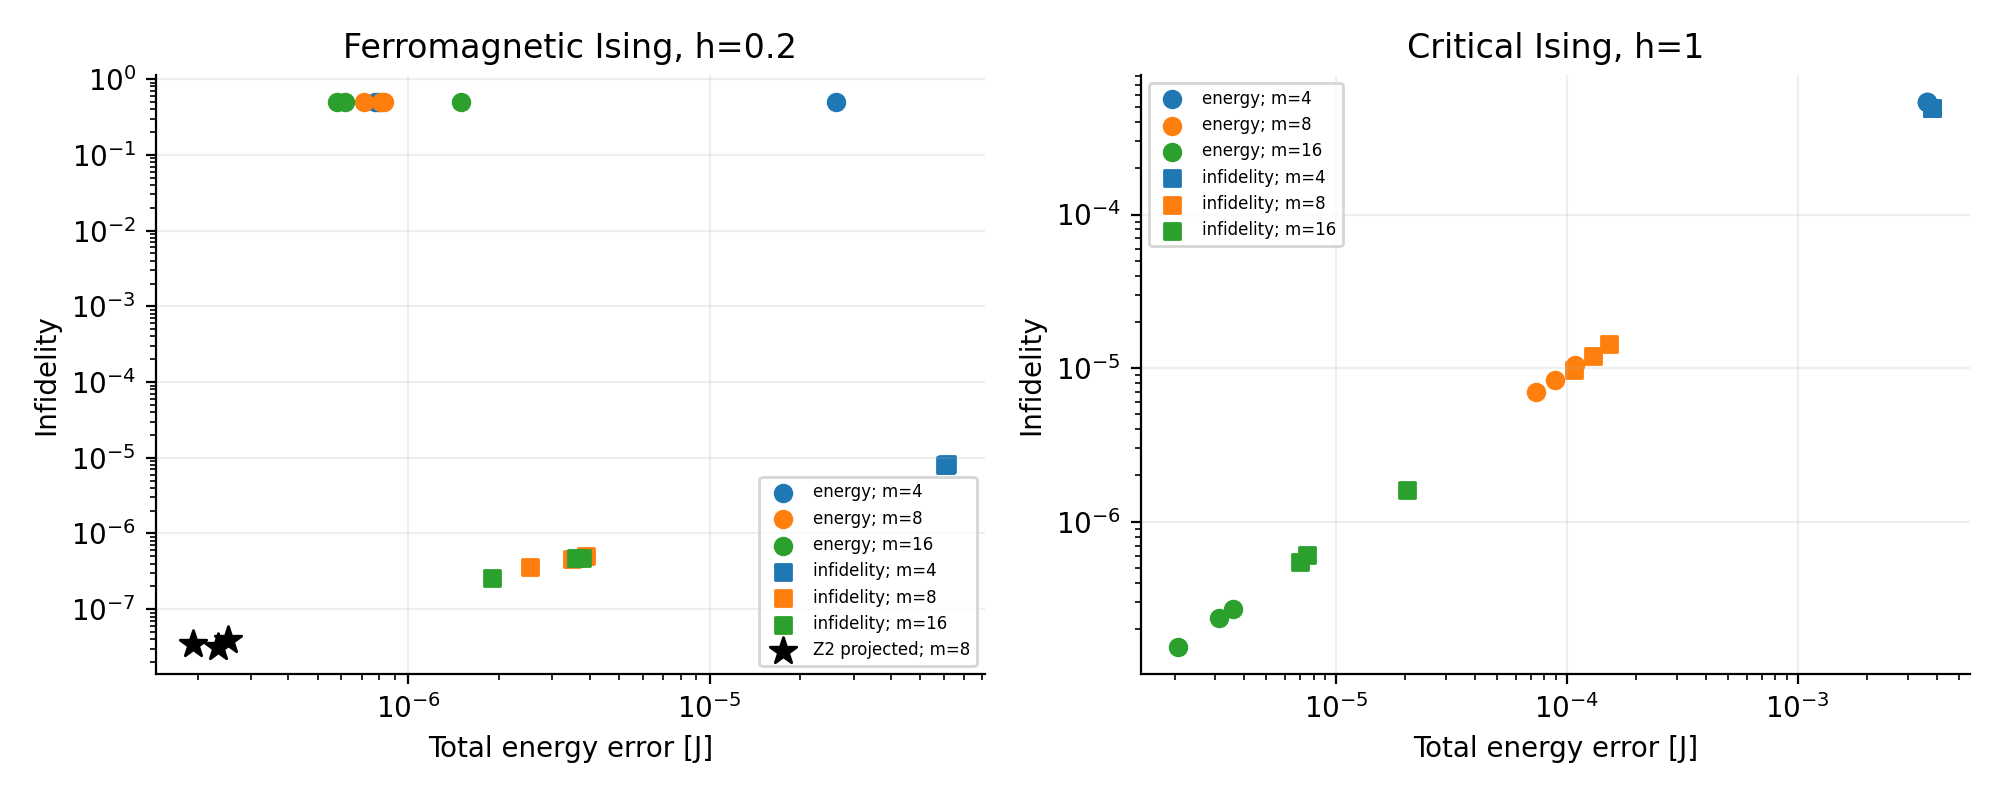
\includegraphics[width=0.95\textwidth,height=\textheight]{figures/energy_fidelity.png}
\caption{Energy error versus infidelity for the eight-site Ising fits.
Colors identify width and markers distinguish the two objectives. The
projected width-eight fits are marked separately in the ordered example.
Three seeds are shown individually. Low energy alone does not identify a
unique target vector near degeneracy.}
\end{figure}

\hypertarget{a-certified-sign-restriction-and-optimization-witnesses}{%
\subsection{5.3 A certified sign restriction and optimization
witnesses}\label{a-certified-sign-restriction-and-optimization-witnesses}}

\par\medskip
\noindent\begin{minipage}{\linewidth}

\textbf{Table 3. Frustrated eight-site chain in the Marshall basis.}
Three-seed means and standard deviations are reported. The
nonnegative-family infidelity bound of 0.5 applies to the RBM rows, not
to the signed network.

\begin{tabular}{@{}lllll@{}}
\toprule\noalign{}
Family & Width & Objective & Energy error & Infidelity \\
\midrule\noalign{}


RBM & 4 & energy & 0.29 (0.16) & 0.582 (0.05) \\
RBM & 4 & infidelity & 0.779 (0.22) & 0.629 (0.074) \\
RBM & 8 & energy & 0.405 (0.16) & 0.617 (0.05) \\
RBM & 8 & infidelity & 0.847 (0.46) & 0.639 (0.14) \\
RBM & 16 & energy & 0.405 (0.16) & 0.617 (0.05) \\
RBM & 16 & infidelity & 0.953 (0.6) & 0.663 (0.18) \\
MLP & 4 & energy & 0.491 (0.26) & 0.718 (0.22) \\
MLP & 4 & infidelity & 0.551 (0.052) & 0.241 (0.017) \\
MLP & 8 & energy & 0.0552 (0.035) & 0.325 (0.25) \\
MLP & 8 & infidelity & 0.00395 (0.0014) & 0.00144 (0.00063) \\
MLP & 16 & energy & 1.73e-13 (1.3e-13) & 4.29e-13 (4.5e-13) \\
MLP & 16 & infidelity & 0.000258 (0.00036) & 0.000114 (0.00016) \\
\bottomrule
\end{tabular}
\end{minipage}\par\medskip


No positive RBM fit violates the analytic bound. Increasing its width
cannot remove that specific sign obstruction, although it can still
change the quality and difficulty of optimization within the allowed
family. Some runs remain far above the lower bound, which does not imply
that the bound is attainable by a finite RBM of that width.

The signed width-sixteen network reaches the reference energy to
approximately \(10^{-13}J\) in the energy fits. Thus the physical target
is accessible to a tested signed family. Width-eight signed energy fits
are much less reliable, but supervised-fit parameters at the same width
provide better energies. The matched lower bounds on their optimization
shortfalls are seed 0: 0.008749J, seed 1: 0.05511J, seed 2: 0.08988J.
These are constructive statements about attained parameters and do not
require solving the global variational problem.

The reverse caution also matters. At width sixteen, energy fits
outperform the retained supervised fits in both mean energy and mean
infidelity. Supervised fitting is therefore a useful intervention, not
an oracle that automatically reveals the representation floor. Reporting
its loss as that floor would incorrectly attribute some optimization
failures to the ansatz.

The sign restriction is basis dependent. In a separate \(J_2=0\)
calculation, the Marshall-basis target has no negative sign mass,
whereas the original-basis positive-family lower bound is about 0.452.
At \(J_2=0.7\), both inspected bases have sign masses one half. These
finite-system observations concern the specified basis and target; they
are not a classification of all frustrated quantum states.

\begin{figure}
\centering
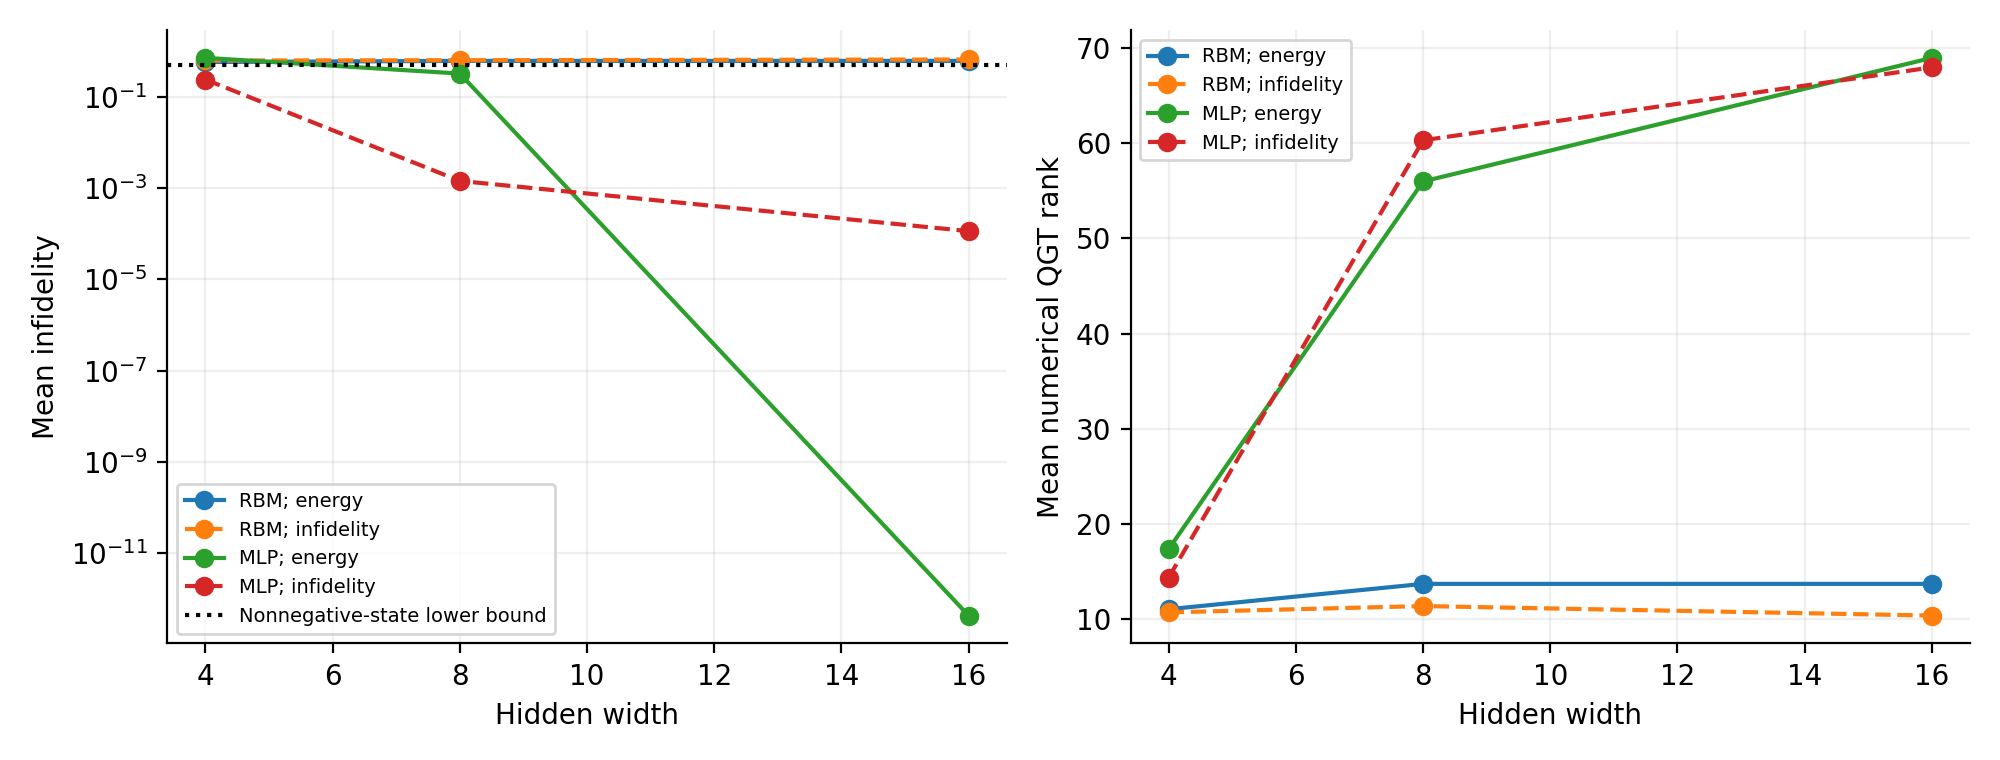
\includegraphics[width=0.95\textwidth,height=\textheight]{figures/sign_restriction.png}
\caption{Frustrated-chain infidelity and thresholded QGT rank versus
hidden width. Lines distinguish objective and family. The horizontal
infidelity bound applies only to nonnegative states. The rank is local
and varies with the achieved state; it is not a certified
representation-capacity curve.}
\end{figure}

\hypertarget{sampler-failure-despite-exact-energy-and-zero-variance}{%
\subsection{5.4 Sampler failure despite exact energy and zero
variance}\label{sampler-failure-despite-exact-energy-and-zero-variance}}

\par\medskip
\noindent\begin{minipage}{\linewidth}

\textbf{Table 4. Frozen exact Ising ground-state sampling.} Each method
has 20 repetitions with 4,096 retained configurations. The reference
magnetization per spin is zero. JSD uses natural logarithms.

\begin{tabular}{@{}
  >{\raggedright\arraybackslash}p{(\columnwidth - 6\tabcolsep) * \real{0.2500}}
  >{\raggedright\arraybackslash}p{(\columnwidth - 6\tabcolsep) * \real{0.2500}}
  >{\raggedright\arraybackslash}p{(\columnwidth - 6\tabcolsep) * \real{0.2500}}
  >{\raggedright\arraybackslash}p{(\columnwidth - 6\tabcolsep) * \real{0.2500}}@{}}
\toprule\noalign{}
\begin{minipage}[b]{\linewidth}\raggedright
Sampler
\end{minipage} & \begin{minipage}[b]{\linewidth}\raggedright
Mean absolute magnetization error
\end{minipage} & \begin{minipage}[b]{\linewidth}\raggedright
Mean JSD
\end{minipage} & \begin{minipage}[b]{\linewidth}\raggedright
Runs with no sign change
\end{minipage} \\
\midrule\noalign{}


iid & 0.01114 & 0.0008939 & 0 \\
local\_up & 0.9947 & 0.2164 & 20 \\
local\_down & 0.9947 & 0.2164 & 20 \\
global\_flip & 0.01672 & 0.001408 & 0 \\
\bottomrule
\end{tabular}
\end{minipage}\par\medskip


Every local-up and local-down repetition remains in its initial
magnetization sector. Their mean magnetizations are approximately
\(+0.995\) and \(-0.995\), respectively, even though the exact
expectation is zero. The empirical distribution misses roughly half the
target probability mass. Independent draws and whole-chain proposals
recover much smaller magnetization errors under the same retained-sample
count.

Nevertheless, the mean local-energy estimate is correct to numerical
precision for all methods, and observed local-energy variances are of
order \(10^{-30}J^2\). This follows directly from the exact eigenstate
identity \(E_{\rm loc}(\sigma)=E_0\) wherever the state has support. A
biased sampler cannot be diagnosed from the fluctuations of a constant
observable.

The naive within-chain standard error of magnetization is about
\(5.1\times10^{-4}\) for the trapped chains, vastly smaller than their
order-one error. That number is not an appropriate uncertainty estimate
for the global mean. Its failure motivates checking mode-sensitive
observables and distinct initializations rather than inferring mixing
from energy stability.

A simple symmetry audit, \(|\widehat{\langle M\rangle}|>0.1\), flags all
20 trapped repetitions from each initialization and none of the
independent/global-flip repetitions in this experiment. The threshold is
an illustrative diagnostic, not a calibrated hypothesis test. When the
\emph{current trial state} is known to be exactly even, the zero
odd-observable expectation follows without exact diagonalization. For an
unprojected asymmetric trial state, imposing zero magnetization as a
sampler truth would be incorrect.

\begin{figure}
\centering
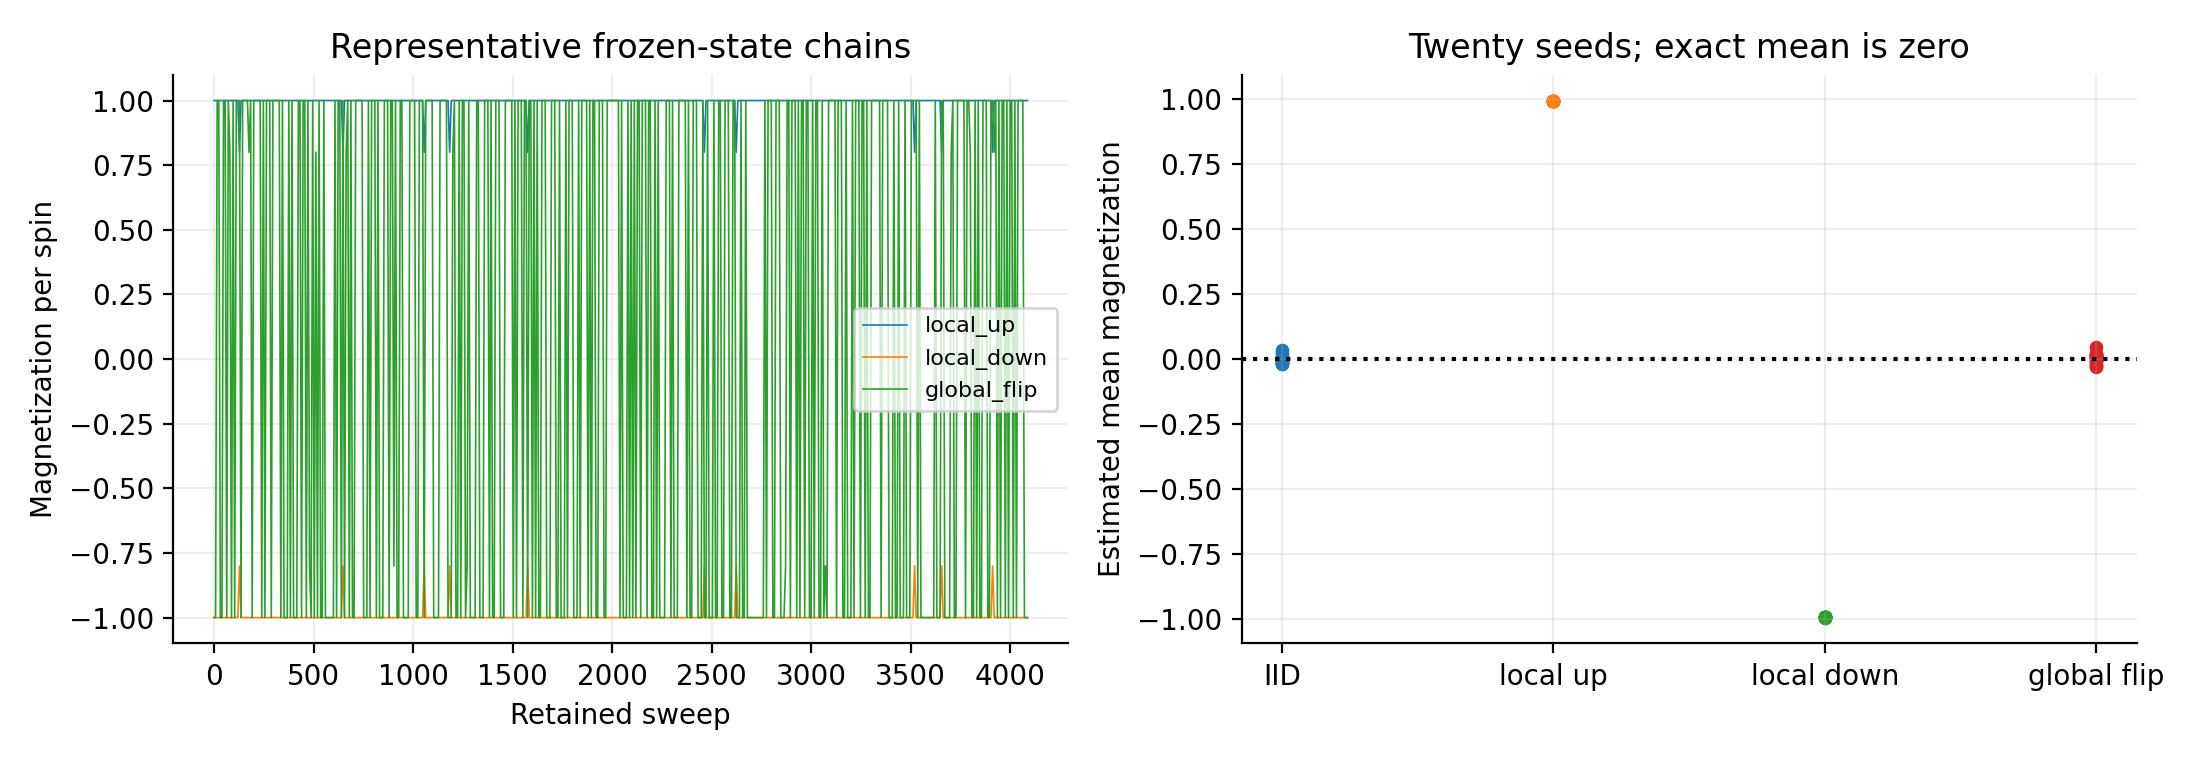
\includegraphics[width=0.95\textwidth,height=\textheight]{figures/sampling.png}
\caption{Representative retained magnetization traces and the estimated
mean magnetization across twenty seeds. The local chains sample opposite
modes depending on initialization. Whole-chain proposals restore mode
changes. Every sampler here uses the same frozen exact state; none of
these differences can be attributed to neural optimization.}
\end{figure}

\hypertarget{finite-sample-rank-is-not-representation-rank}{%
\subsection{5.5 Finite-sample rank is not representation
rank}\label{finite-sample-rank-is-not-representation-rank}}

\par\medskip
\noindent\begin{minipage}{\linewidth}

\textbf{Table 5. Sampled metric ranks at checkpoint 25.} The exact
metric rank is 80 in the reference coordinates. The count of distinct
configurations provides a tighter rank limit than sample count in some
batches.

\begin{tabular}{@{}
  >{\raggedright\arraybackslash}p{(\columnwidth - 8\tabcolsep) * \real{0.2000}}
  >{\raggedright\arraybackslash}p{(\columnwidth - 8\tabcolsep) * \real{0.2000}}
  >{\raggedright\arraybackslash}p{(\columnwidth - 8\tabcolsep) * \real{0.2000}}
  >{\raggedright\arraybackslash}p{(\columnwidth - 8\tabcolsep) * \real{0.2000}}
  >{\raggedright\arraybackslash}p{(\columnwidth - 8\tabcolsep) * \real{0.2000}}@{}}
\toprule\noalign{}
\begin{minipage}[b]{\linewidth}\raggedright
Samples
\end{minipage} & \begin{minipage}[b]{\linewidth}\raggedright
Distinct configurations
\end{minipage} & \begin{minipage}[b]{\linewidth}\raggedright
Metric rank
\end{minipage} & \begin{minipage}[b]{\linewidth}\raggedright
Relative metric error
\end{minipage} & \begin{minipage}[b]{\linewidth}\raggedright
Relative gradient error
\end{minipage} \\
\midrule\noalign{}


16 & 10.5 (1.8) & 9.5 (1.8) & 0.6027 & 5.471 \\
64 & 30.5 (3.5) & 29.5 (3.5) & 0.3052 & 2.871 \\
256 & 76.7 (5.3) & 74.9 (4.3) & 0.1549 & 1.453 \\
1024 & 147 (6.2) & 80 (0) & 0.07662 & 0.7361 \\
\bottomrule
\end{tabular}
\end{minipage}\par\medskip


A low sampled rank can arise solely because too few configurations were
observed. In the experiment the underlying neural family, frozen
parameters, and exact metric remain unchanged. Interpreting that sampled
rank as a reduction in intrinsic representation capacity would therefore
be a category error.

The local-tangent limitation is different again. The positive log-table
example has full local rank 69 in the frustrated sector and still has
the proven sign-induced infidelity floor. Together these examples show
why a rank statistic needs a declared object: population or sampled
metric, numerical or formal rank, fixed parametrization or rescaled
coordinates, and local or global representability.

\hypertarget{noisy-metric-and-gradient-interact}{%
\subsection{5.6 Noisy metric and gradient
interact}\label{noisy-metric-and-gradient-interact}}

\par\medskip
\noindent\begin{minipage}{\linewidth}

\textbf{Table 6. Matched metric/gradient interventions at checkpoint
25.} The ridge is \(10^{-3}\bar s\) and the true linearized displacement
is 0.002. Entries are percentages of uphill directions or finite steps
over 100 batches, and mean direction cosine to the population reference.

\begin{tabular}{@{}
  >{\raggedright\arraybackslash}p{(\columnwidth - 8\tabcolsep) * \real{0.2000}}
  >{\raggedright\arraybackslash}p{(\columnwidth - 8\tabcolsep) * \real{0.2000}}
  >{\raggedright\arraybackslash}p{(\columnwidth - 8\tabcolsep) * \real{0.2000}}
  >{\raggedright\arraybackslash}p{(\columnwidth - 8\tabcolsep) * \real{0.2000}}
  >{\raggedright\arraybackslash}p{(\columnwidth - 8\tabcolsep) * \real{0.2000}}@{}}
\toprule\noalign{}
\begin{minipage}[b]{\linewidth}\raggedright
Samples
\end{minipage} & \begin{minipage}[b]{\linewidth}\raggedright
Intervention
\end{minipage} & \begin{minipage}[b]{\linewidth}\raggedright
Linear uphill (\%)
\end{minipage} & \begin{minipage}[b]{\linewidth}\raggedright
Finite uphill (\%)
\end{minipage} & \begin{minipage}[b]{\linewidth}\raggedright
Direction cosine
\end{minipage} \\
\midrule\noalign{}


16 & population & 0 & 0 & 1 \\
16 & metric only noise & 0 & 0 & 0.2923 \\
16 & gradient only noise & 0 & 0 & 0.2576 \\
16 & joint ridge & 28 & 33 & 0.0389 \\
256 & population & 0 & 0 & 1 \\
256 & metric only noise & 0 & 0 & 0.704 \\
256 & gradient only noise & 0 & 0 & 0.7357 \\
256 & joint ridge & 0 & 0 & 0.8049 \\
\bottomrule
\end{tabular}
\end{minipage}\par\medskip


With the true gradient, a regularized positive-definite sampled metric
cannot produce a first-order uphill direction; the observed zero rate is
consistent with that algebraic identity. Gradient replacement alone also
produces no first-order uphill directions in these retained batches,
although it changes directions and can affect finite steps.

Replacing both quantities can produce uphill directions at small sample
count. The phenomenon is therefore not adequately described as the
metric having become indefinite: the regularized metric remains positive
definite. The estimated gradient and the geometry used to precondition
it jointly determine alignment with the true energy gradient. Increasing
samples reduces this particular failure in the tested checkpoints,
without implying a universal sample threshold for other states.

Alternative ridge strengths, a diagonal shift, and a parameter-group
block approximation are all retained in the raw records. They can
improve one-step behavior relative to an excessively small shift, but no
single approximation is established as best over systems or training
stages. The present scale is too small to evaluate a computational
scalability advantage.

\begin{figure}
\centering
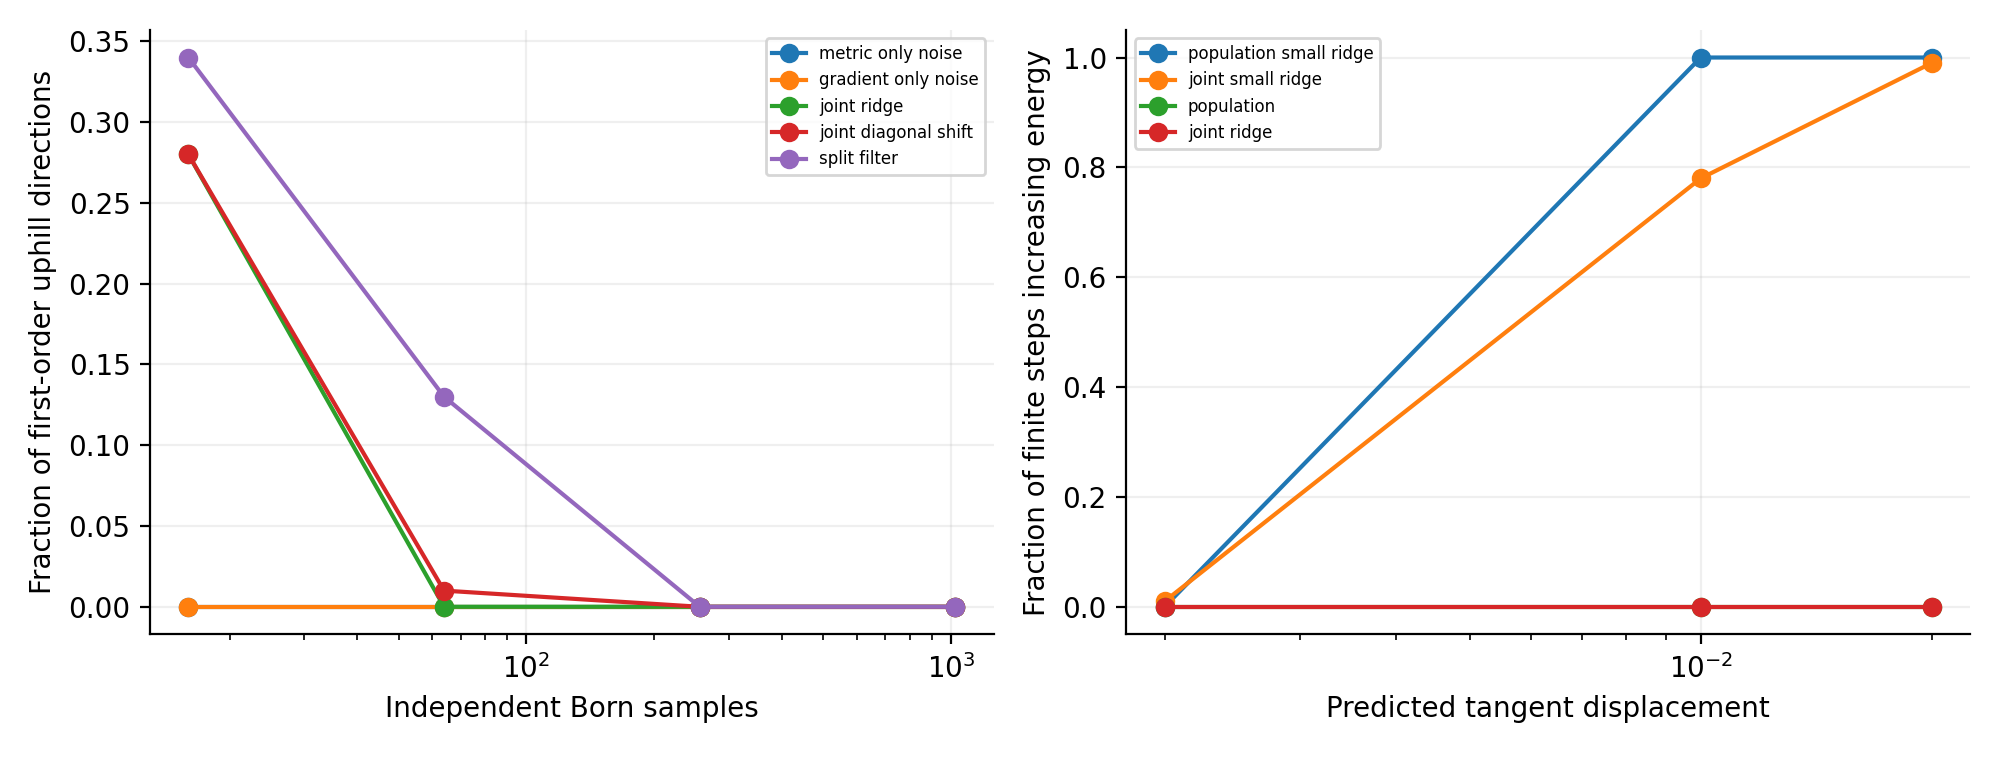
\includegraphics[width=0.95\textwidth,height=\textheight]{figures/qgt_noise.png}
\caption{Left: first-order uphill fractions under independent
metric/gradient interventions at checkpoint 25. Right: finite-step
uphill fractions as the intended tangent displacement increases, with
matched deterministic and sampled small-shift controls. Sampling error
and nonlinear overshoot are separate mechanisms.}
\end{figure}

\hypertarget{a-descent-direction-is-not-a-finite-step-guarantee}{%
\subsection{5.7 A descent direction is not a finite-step
guarantee}\label{a-descent-direction-is-not-a-finite-step-guarantee}}

\par\medskip
\noindent\begin{minipage}{\linewidth}

\textbf{Table 7. Weak-ridge linearization control at checkpoint 25.} The
ridge is \(10^{-6}\bar s\). Sampled cases use 256 configurations. The
actual distance is the mean phase-invariant chord distance;
deterministic rows describe one fixed direction, repeated in the data
structure for matching.

\begin{tabular}{@{}
  >{\raggedright\arraybackslash}p{(\columnwidth - 8\tabcolsep) * \real{0.2000}}
  >{\raggedright\arraybackslash}p{(\columnwidth - 8\tabcolsep) * \real{0.2000}}
  >{\raggedright\arraybackslash}p{(\columnwidth - 8\tabcolsep) * \real{0.2000}}
  >{\raggedright\arraybackslash}p{(\columnwidth - 8\tabcolsep) * \real{0.2000}}
  >{\raggedright\arraybackslash}p{(\columnwidth - 8\tabcolsep) * \real{0.2000}}@{}}
\toprule\noalign{}
\begin{minipage}[b]{\linewidth}\raggedright
Intended distance
\end{minipage} & \begin{minipage}[b]{\linewidth}\raggedright
Update
\end{minipage} & \begin{minipage}[b]{\linewidth}\raggedright
Linear uphill (\%)
\end{minipage} & \begin{minipage}[b]{\linewidth}\raggedright
Finite uphill (\%)
\end{minipage} & \begin{minipage}[b]{\linewidth}\raggedright
Actual chord
\end{minipage} \\
\midrule\noalign{}


0.002 & population & 0 & 0 & 0.004424 \\
0.002 & sampled & 0 & 1 & 0.003426 \\
0.01 & population & 0 & 100 & 0.1105 \\
0.01 & sampled & 0 & 78 & 0.07107 \\
0.02 & population & 0 & 100 & 0.4378 \\
0.02 & sampled & 0 & 99 & 0.273 \\
\bottomrule
\end{tabular}
\end{minipage}\par\medskip


At intended displacement 0.02, the deterministic weak-ridge step changes
the state by a chord distance about 0.438 and increases energy, despite
being a true first-order descent direction. This is a failure of the
local linearized step to predict the nonlinear displacement. It exists
without sampling and therefore cannot be counted as evidence of a Monte
Carlo failure.

Reducing the intended displacement to 0.002 eliminates deterministic
overshoot for that control. The sampled weak-ridge update still has
occasional finite-step failures, while larger-shift variants are more
stable in this example. The result supports inspecting actual changes in
the state and using finite-step safeguards, rather than attributing
every unstable SR update to noisy eigenvalues.

\hypertarget{coordinate-dependence-of-numerical-rank-and-regularization}{%
\subsection{5.8 Coordinate dependence of numerical rank and
regularization}\label{coordinate-dependence-of-numerical-rank-and-regularization}}

\par\medskip
\noindent\begin{minipage}{\linewidth}

\textbf{Table 8. Positive diagonal parameter rescaling at a fixed
state.} The physical family and formal tangent dimension are unchanged.
Direction cosines compare each update with its own unscaled counterpart.

\begin{tabular}{@{}
  >{\raggedright\arraybackslash}p{(\columnwidth - 8\tabcolsep) * \real{0.2000}}
  >{\raggedright\arraybackslash}p{(\columnwidth - 8\tabcolsep) * \real{0.2000}}
  >{\raggedright\arraybackslash}p{(\columnwidth - 8\tabcolsep) * \real{0.2000}}
  >{\raggedright\arraybackslash}p{(\columnwidth - 8\tabcolsep) * \real{0.2000}}
  >{\raggedright\arraybackslash}p{(\columnwidth - 8\tabcolsep) * \real{0.2000}}@{}}
\toprule\noalign{}
\begin{minipage}[b]{\linewidth}\raggedright
Scale extent (decades)
\end{minipage} & \begin{minipage}[b]{\linewidth}\raggedright
Raw rank
\end{minipage} & \begin{minipage}[b]{\linewidth}\raggedright
Normalized rank
\end{minipage} & \begin{minipage}[b]{\linewidth}\raggedright
Isotropic cosine
\end{minipage} & \begin{minipage}[b]{\linewidth}\raggedright
Diagonal-shift cosine
\end{minipage} \\
\midrule\noalign{}


0.0 & 80 & 80 & 1 & 1 \\
1.0 & 79 & 80 & 0.942 & 1 \\
3.0 & 45 & 80 & 0.4464 & 1 \\
6.0 & 24 & 80 & 0.3018 & 1 \\
\bottomrule
\end{tabular}
\end{minipage}\par\medskip


The raw thresholded rank falls from 80 to 24, while the
column-normalized rank remains 80. This is not a loss of physical
directions: the coordinate transformation is invertible. Isotropic
trace-scaled ridge also changes the physical update substantially,
because adding an identity matrix introduces a parameter-coordinate
convention.

The diagonal-shift update agrees with its unscaled physical parameter
step to relative differences below approximately \(2\times10^{-13}\) in
the tested rescalings. That agreement follows from its covariance under
positive diagonal transformations, and is supported numerically by a
preconditioned solve. It does not make the method invariant under
arbitrary parameter mixing, nonlinear changes of variables, or sample
noise. A small isotropic numerical floor can also break exact
covariance; it is not used in this idealized identity test.

\begin{figure}
\centering
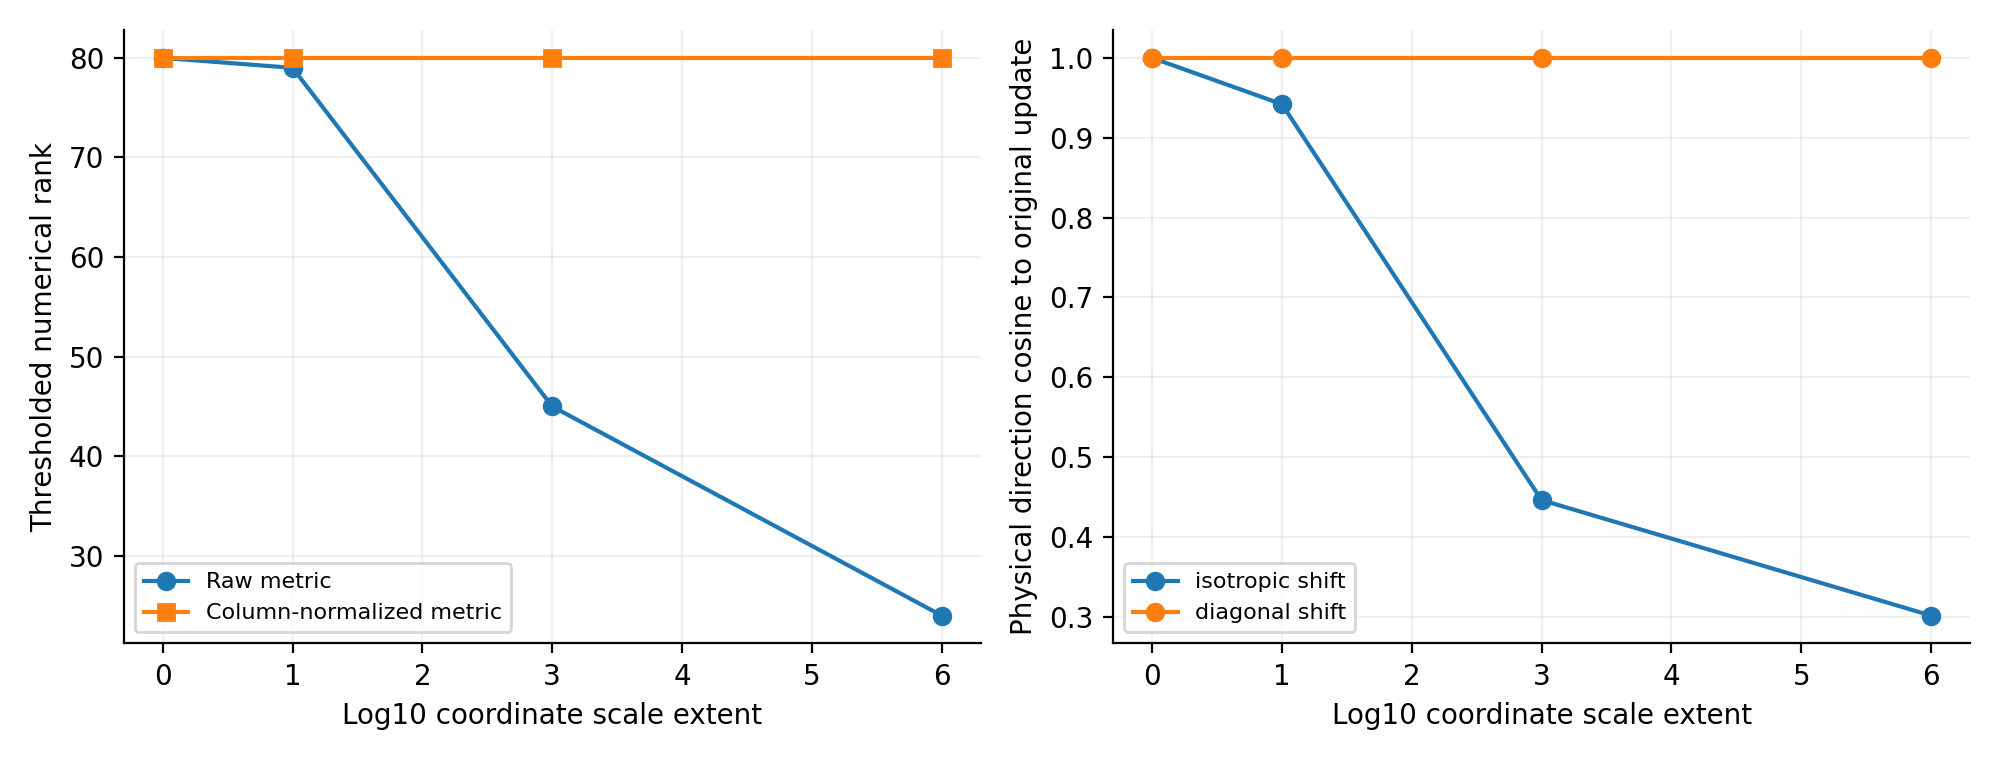
\includegraphics[width=0.95\textwidth,height=\textheight]{figures/coordinates.png}
\caption{Thresholded rank and physical update direction under coordinate
rescaling. The column-normalized metric removes this diagonal-scaling
dependence, while the isotropic shifted update changes direction. These
are numerical-coordinate controls, not changes in the represented
quantum state.}
\end{figure}

\hypertarget{an-exploratory-filter-that-is-not-consistently-useful}{%
\subsection{5.9 An exploratory filter that is not consistently
useful}\label{an-exploratory-filter-that-is-not-consistently-useful}}

The split-sample heuristic estimates candidate metric eigenvectors on
half a batch, then retains directions only when their variance is within
a factor of four on the second half and their projected gradient
estimates have matching signs. It uses the same total sample count and
population-scale ridge as the reference comparison. Appendix C gives the
rule explicitly.

This heuristic is not a robust improvement. At checkpoint 25 and 64
samples, its first-order uphill rate is 13\%, compared with 0\% for the
matched ordinary joint ridge. At larger sample counts it improves but
still does not establish an advantage. Splitting a small batch
sacrifices information, and directional sign agreement is too weak a
guarantee of alignment with the population gradient. The current
heuristic is therefore retained as a negative result rather than
promoted as a new optimization method. Statistical filtering and
independent-batch validation already have substantial prior context
{[}6{]}.

\hypertarget{exact-sum-optimizer-comparisons}{%
\subsection{5.10 Exact-sum optimizer
comparisons}\label{exact-sum-optimizer-comparisons}}

\par\medskip
\noindent\begin{minipage}{\linewidth}

\textbf{Table 9. Exact-sum optimization from matched initializations,
width eight.} Each method allows 500 update steps. Energy and infidelity
are seed means; Hamiltonian-vector counts include recorded line-search
trials. Counts are not runtime or equal-cost guarantees.

\begin{tabular}{@{}lllll@{}}
\toprule\noalign{}
Coupling & Optimizer & Energy error & Infidelity & H-vector calls \\
\midrule\noalign{}


h=0.2 & Adam & 0.0001364 & 0.4974 & 500 \\
h=0.2 & SR isotropic & 9.285e-07 & 0.004881 & 1000 \\
h=0.2 & SR diagonal & 5.665e-07 & 0.004795 & 1000 \\
h=0.2 & SR block & 7.737e-07 & 0.3819 & 1075 \\
h=1 & Adam & 0.0008597 & 9.221e-05 & 500 \\
h=1 & SR isotropic & 8.397e-05 & 8.068e-06 & 1000 \\
h=1 & SR diagonal & 0.0001009 & 9.385e-06 & 1000 \\
h=1 & SR block & 0.00011 & 1.141e-05 & 1035 \\
\bottomrule
\end{tabular}
\end{minipage}\par\medskip


SR improves the critical-chain energy substantially relative to the
retained Adam settings. In the ordered chain, the full-metric SR
variants also find much better target fidelities than Adam or the block
approximation in these runs. Their energy differences are much less
dramatic because of the small gap. These outcomes reinforce the need to
report the target state or observable alongside energy.

The SR implementations use exact sums and an exact-energy Armijo
backtracking test, with caps on predicted tangent displacement and
parameter-step norm. Their stability cannot be credited solely to the
metric, and the comparison is not a benchmark against tuned production
implementations. The displayed Hamiltonian-vector counts omit different
costs of Jacobian construction and metric solves. No end-to-end
wall-clock speedup is inferred.

\begin{figure}
\centering
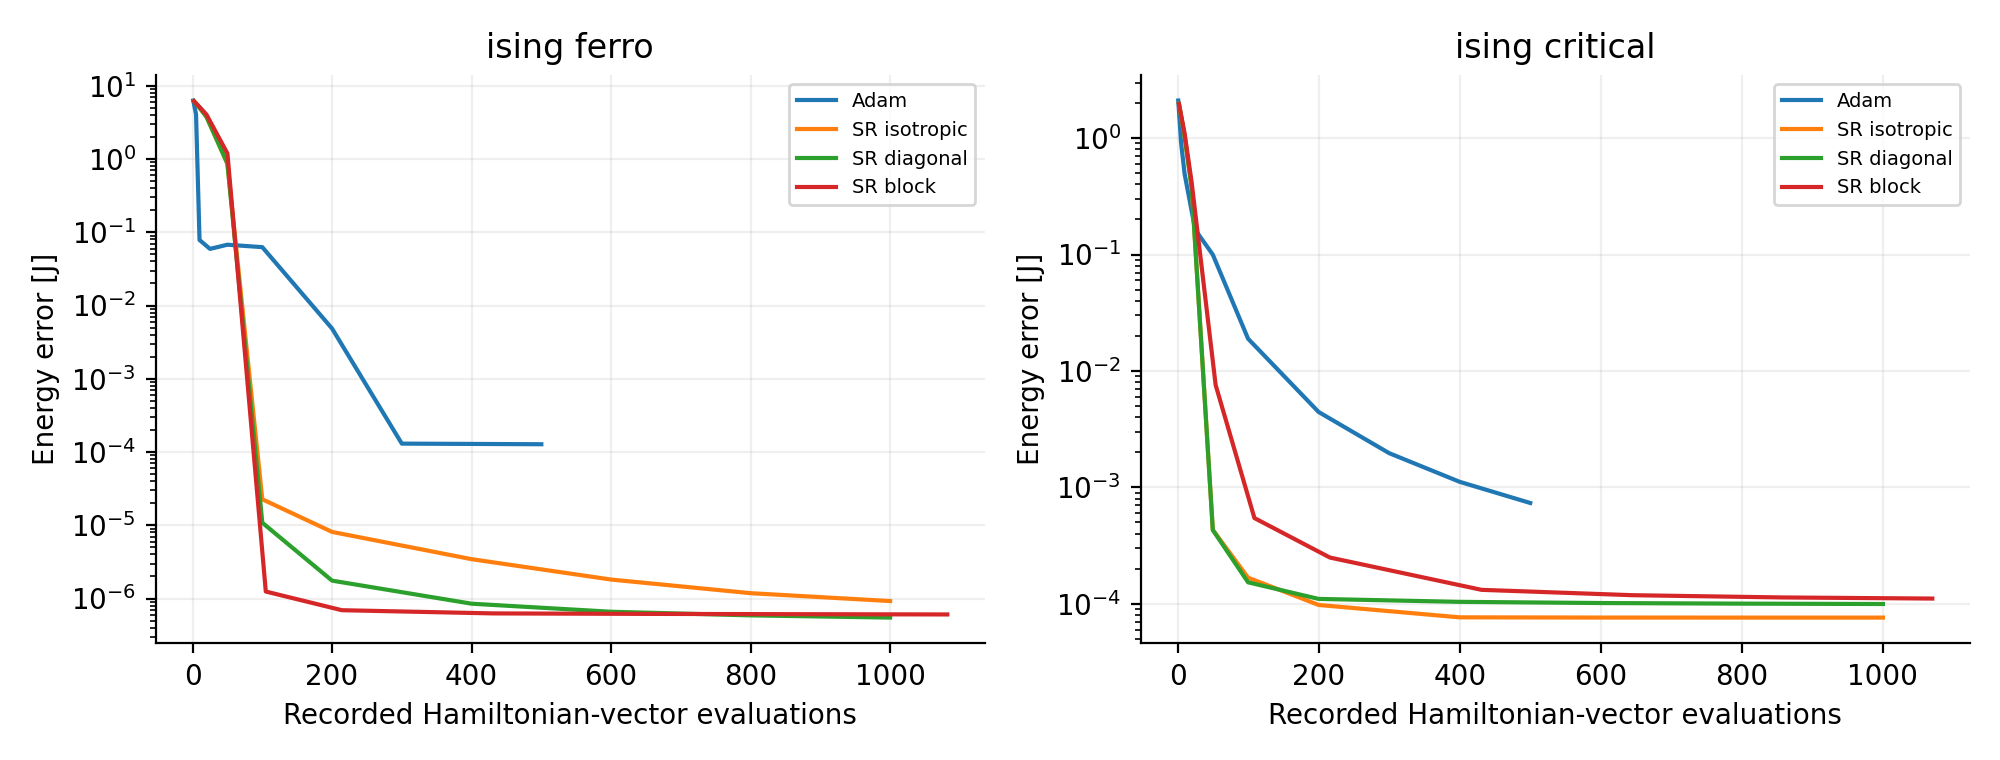
\includegraphics[width=0.95\textwidth,height=\textheight]{figures/optimizers.png}
\caption{Representative seed-zero exact-sum optimization traces versus
recorded Hamiltonian-vector evaluations. The comparisons use stated
fixed hyperparameters and do not constitute equal-runtime studies. Both
fields use an eight-hidden-unit RBM.}
\end{figure}

\hypertarget{discussion}{%
\section{6. Discussion}\label{discussion}}

\hypertarget{a-diagnosis-should-identify-an-intervention}{%
\subsection{6.1 A diagnosis should identify an
intervention}\label{a-diagnosis-should-identify-an-intervention}}

The strongest statements in this study are constructive. A sign-mass
bound certifies that the nonnegative family cannot approximate the
selected frustrated target beyond a known fidelity. A lower-energy
parameter vector in the same family certifies that a particular energy
run has an optimization shortfall. Holding the exact wavefunction fixed
while changing only the sampler isolates mixing errors. Holding the
checkpoint fixed while independently replacing metric and gradient
estimates isolates sources of update error.

These tests do not yield a universal automatic classifier. Several
mechanisms can coexist, and evidence about one does not exclude the
others. A positive RBM can have both a sign obstruction and a poor
optimization within its allowed orthant. A sampled update can suffer
both gradient-estimation error and nonlinear overshoot. A low-gap
objective can legitimately produce a useful low-energy state whose
fidelity is unsatisfactory for a separate target-state task.

The practical sequence is therefore to ask what information would change
the next action. A proven sign restriction calls for a different
phase/sign representation or basis. A constructive lower-energy witness
calls for an optimizer or initialization investigation. A frozen-state
discrepancy between samplers calls for sampling changes. A gap-sensitive
fidelity problem calls for a better specified state sector, observable,
or objective. A raw rank statistic alone does not select among these
actions.

\hypertarget{what-the-qgt-can-and-cannot-diagnose}{%
\subsection{6.2 What the QGT can and cannot
diagnose}\label{what-the-qgt-can-and-cannot-diagnose}}

The QGT is an informative local geometric object. It quantifies state
changes under parameter variations and underlies useful natural-gradient
updates. Its singular directions can identify locally redundant
parameter combinations, and its tangent image can reveal which part of
an imaginary-time residual is currently accessible.

That local information must be interpreted with its statistical and
coordinate context. A sampled metric can lose rank because only a few
configurations were seen. A thresholded population spectrum can change
under parameter rescaling. A full local tangent dimension can coexist
with a global sign restriction. A large parameter update along a weakly
visible tangent direction can invalidate the linearized geometry. None
of these observations makes the QGT unhelpful; they specify the controls
required to use it responsibly.

The practical recommendation is to report the normalized-state Jacobian
or its equivalent metric convention, rank thresholds, sample and
distinct-configuration counts, and both absolute and relative tangent
residuals. When comparing regularizers, physical state changes and
independent energy evaluations are more informative than parameter-step
norms alone. These are reporting and diagnostic recommendations
supported at small scale, not a new large-system optimizer.

\hypertarget{three-project-specific-directions-worth-pursuing}{%
\subsection{6.3 Three project-specific directions worth
pursuing}\label{three-project-specific-directions-worth-pursuing}}

The following proposals are original to this research plan, not
assertions of priority over existing literature.

First, symmetry identities can provide inexpensive sampler audits when
energy is uninformative. If the trial family enforces a symmetry,
observables odd under that symmetry have known zero expectation without
exact diagonalization. Several such identities, paired chains, and
sector-crossing counts could form a useful audit suite. The key
qualification is that the identity must hold for the \emph{current trial
state}, not merely for the desired exact ground state. The frozen
example demonstrates the principle; calibration during large-system
training remains untested.

Second, a persistent bank of best-known parameter witnesses could make
optimization diagnoses less dependent on a single training objective. In
exact small systems, the energy comparison is direct. In sampled
calculations, paired independent energy estimates and their uncertainty
would be needed before declaring one parameter vector a better witness.
Such a bank would bound optimizer shortfall from below without
pretending to identify the global representation error. The present
archive provides a small exact example, not a general inference
procedure.

Third, finite-step safeguards could test the actual state overlap rather
than rely only on a linearized QGT norm. The weak-ridge control shows a
large discrepancy between predicted and actual displacement even with
exact statistics. An independent overlap estimate could therefore
complement energy backtracking in a sampled optimizer. Whether it is
reliable and affordable depends on its own estimator variance and
support coverage. No scalable overlap-based trust-region algorithm is
demonstrated here.

\hypertarget{relationship-to-the-earlier-electronic-state-study}{%
\subsection{6.4 Relationship to the earlier electronic-state
study}\label{relationship-to-the-earlier-electronic-state-study}}

The preceding molecular study emphasized that accurate scalar energy and
a consistent local derivative construction do not automatically certify
another observable. The present spin study identifies analogous
distinctions for state fidelity, sampling, and tangent geometry. The
implementations are separate: no molecular result is used as spin
reference data, and no claim of transfer from electronic coefficients to
the spin ansätze is made.

The methodological continuity is the use of exact small systems as a
control, followed by interventions that expose the limits of a
diagnostic. The next substantial extension should preserve those
controls while introducing a larger configuration-conditioned model and
actual sampled training. Simply scaling the current dense geometry
diagnostics would not establish that the same conclusions dominate
production variational Monte Carlo.

\hypertarget{limitations}{%
\section{7. Limitations}\label{limitations}}

The Hamiltonians are small one-dimensional spin models. Most systems
have eight sites, with a ten-site state used for one training comparison
and another for frozen sampling. There is no two-dimensional magnet,
thermodynamic extrapolation, molecular simulation, or application to an
experimentally unresolved phase. The sign obstruction concerns a real
positive ansatz in a stated computational basis, not complex neural
states in arbitrary bases.

The exact-sum training and supervised fits have finite budgets and only
three initialization seeds. Many reach the cap, and successful numerical
termination is not a global-optimality certificate. Supervised fitting
uses exact labels and can be worse than energy fitting. The proven
representation claim is limited to the sign-mass bound; all other
achieved losses are finite-budget observations.

The sampling study freezes an exact ground state. Its energy estimator
is deliberately an extreme zero-variance control. Actual imperfect
states generally have nonconstant local energy, and local-energy
diagnostics can then reveal some failures. The experiment proves that
those diagnostics are insufficient in general, not that they are
useless. Up/down trajectories use paired seeds, and no claim is made
that a short global-flip repair handles more complicated multimodal
distributions.

The stochastic metric study uses independent exact Born samples and only
two checkpoints from one trajectory. It does not include MCMC
autocorrelation in the metric/gradient batches. The shift scale and step
normalization use population quantities available only in this
diagnostic. Thus the one-step results are not deployment performance
estimates or end-to-end sampled-training claims. The filter comparison
has no extensive tuning or broader benchmark validation.

Coordinate invariance is tested only for positive diagonal rescaling.
Column normalization and diagonal shifts do not solve arbitrary
reparametrization problems. Numerical rank and tangent residuals require
stated tolerances. The exact-sum optimizer comparison includes oracle
energy line searches and different costs per update, so its iteration
counts cannot establish a runtime advantage.

The literature already contains representation/sampling studies, QGT
diagnostics, symmetry projection, and statistical SR regularization. The
contribution of this report is a transparent collection of validated
interventions and their measured outcomes. It does not claim a new
representation theorem, a new universal failure taxonomy, or a
state-of-the-art optimizer.

\hypertarget{conclusion}{%
\section{8. Conclusion}\label{conclusion}}

A stalled neural quantum-state calculation requires more than one
diagnostic. In controlled small spin systems, we distinguish an
analytically proven sign restriction, optimization shortfalls certified
by attainable parameter witnesses, mode-trapped sampling despite exact
energy estimates, and objective sensitivity caused by a very small
finite-size gap.

The QGT provides useful local geometry but does not by itself identify
the mechanism. Its sampled rank can reflect observation count, its
numerical spectrum can reflect parameter scaling, and its linearized
norm can underestimate finite nonlinear state changes. Matched
interventions separate noisy directions from deterministic overshoot,
while the unsuccessful split-sample filter illustrates why a plausible
diagnostic heuristic should be tested before being promoted.

The resulting research direction is concrete: combine physical-sector
information, independent sampler audits, attainable-state witnesses, and
measured state displacements. These controls offer a defensible
foundation for larger sampled calculations, where the same questions
become harder precisely because exact reference states are no longer
available.

\hypertarget{references}{%
\section{References}\label{references}}

\begin{enumerate}
\def\labelenumi{\arabic{enumi}.}
\tightlist
\item
  G. Carleo and M. Troyer. \emph{Solving the quantum many-body problem
  with artificial neural networks}. Science \textbf{355}, 602--606
  (2017). https://doi.org/10.1126/science.aag2302. Preprint:
  https://arxiv.org/abs/1606.02318.
\item
  C.-Y. Park and M. J. Kastoryano. \emph{Expressive power of
  complex-valued restricted Boltzmann machines for solving
  non-stoquastic Hamiltonians}. Physical Review B \textbf{106}, 134437
  (2022). https://doi.org/10.1103/PhysRevB.106.134437. Preprint:
  https://arxiv.org/abs/2012.08889.
\item
  S. Dash, L. Gravina, F. Vicentini, M. Ferrero, and A. Georges.
  \emph{Efficiency of neural quantum states in light of the quantum
  geometric tensor}. Communications Physics \textbf{8}, 92 (2025).
  https://doi.org/10.1038/s42005-025-02005-4.
\item
  A. Chen and M. Heyl. \emph{Empowering deep neural quantum states
  through efficient optimization}. Nature Physics \textbf{20},
  1476--1481 (2024). https://doi.org/10.1038/s41567-024-02566-1.
\item
  A. Shokry, A. Santini, and F. Vicentini. \emph{When Less is More:
  Approximating the Quantum Geometric Tensor with Block Structures}.
  arXiv:2510.08430 (2025), version 2. https://arxiv.org/abs/2510.08430.
  Preprint.
\item
  T. Hur. \emph{Stochastic Reconfiguration as Statistical Filtering for
  Overparameterized Neural Quantum States}. arXiv:2609.23334v1, 20
  September 2026. https://arxiv.org/abs/2609.23334. Preprint; cited as
  related work, not independently reproduced.
\item
  K. Choo, G. Carleo, N. Regnault, and T. Neupert. \emph{Symmetries and
  Many-Body Excitations with Neural-Network Quantum States}. Physical
  Review Letters \textbf{121}, 167204 (2018).
  https://doi.org/10.1103/PhysRevLett.121.167204.
\item
  E. Ledinauskas and E. Anisimovas. \emph{Neural Importance Resampling:
  A Practical Sampling Strategy for Neural Quantum States}.
  arXiv:2507.20510 (2025). https://arxiv.org/abs/2507.20510. The
  preprint is used for methodological context; its algorithm is not
  reproduced.
\end{enumerate}

\hypertarget{appendix-a.-positivity-bound-and-witness-logic}{%
\section{Appendix A. Positivity bound and witness
logic}\label{appendix-a.-positivity-bound-and-witness-logic}}

Write \(u=u_+-u_-\) with disjoint nonnegative components. For any
nonnegative normalized \(c\), \(u^Tc=u_+^Tc-u_-^Tc\). Its positive value
is at most \(\|u_+\|\) and the magnitude of its negative value is at
most \(\|u_-\|\). Squaring gives \(|u^Tc|^2\le\max(P_+,P_-)\). The
extremal nonnegative vector is the normalized larger sign component.
Strict positivity allows the same supremum only as a limit if the other
component is nonempty.

For any obtained witness \(\theta_w\),
\(\inf_\theta E(\theta)\le E(\theta_w)\). Subtracting from
\(E(\theta_e)\) proves the optimization-shortfall bound. The witness
need not be a ground-state approximation or a supervised optimum. If its
energy is estimated stochastically, finite-sample uncertainty must be
included before declaring a positive bound.

For the positive log-table family, differentiation gives
\(S_{ij}=p_i\delta_{ij}-p_ip_j\). The all-ones vector is null, and
\(x^TSx=\operatorname{Var}_p(x)>0\) for every nonconstant \(x\) when all
\(p_i>0\). Hence its exact rank is \(D-1\), regardless of a global sign
obstruction relative to a target outside the positive orthant.

\hypertarget{appendix-b.-gradient-and-geometric-conventions}{%
\section{Appendix B. Gradient and geometric
conventions}\label{appendix-b.-gradient-and-geometric-conventions}}

All experimental states and parameters are real. The metric is the real
normalized-state QGT; imaginary Berry-curvature components are not
studied. For the RBM, the logarithmic derivatives are
\(O_{a_i}=\sigma_i\), \(O_{b_j}=\tanh z_j\), and
\(O_{W_{ij}}=\sigma_i\tanh z_j\). Subtracting their Born means yields
the normalized tangent. The energy-gradient convention contains a factor
of two; SR matrices and gradients use that convention consistently.

The exact first-order energy change is \(g^T\delta\theta\). The
predicted tangent displacement is
\(\sqrt{\delta\theta^TS\delta\theta}\). The actual distance used in the
tables is

\[d_{\rm chord}(c,c')=\sqrt{2(1-|c^Tc'|)},\]

which removes the unphysical global sign. It agrees with the tangent
norm infinitesimally but need not do so for a finite parameter step. It
is a chord distance between rays, not the exact Fubini--Study angle.

Under \(\theta=D\phi\), \(S_\phi=DSD\) for positive diagonal \(D\).
Adding \(\lambda\operatorname{diag}(S_\phi)\) transforms in the same way
as adding \(\lambda\operatorname{diag}(S)\) before rescaling. An
isotropic \(\lambda I\) generally does not. Column-normalized solves
implement the former identity without relying on numerically
ill-conditioned raw coordinates.

\hypertarget{appendix-c.-exploratory-split-filter-and-optimizer-settings}{%
\section{Appendix C. Exploratory split filter and optimizer
settings}\label{appendix-c.-exploratory-split-filter-and-optimizer-settings}}

The split filter divides each batch equally. It diagonalizes
\(\widehat S_A=U\Lambda U^T\) and evaluates
\(v_i=u_i^T\widehat S_Bu_i\), \(f_{Ai}=u_i^T\widehat g_A\), and
\(f_{Bi}=u_i^T\widehat g_B\). A direction is kept if

\[\lambda_i>10^{-6}\bar s,\quad \lambda_i/4<v_i<4\lambda_i,\quad f_{Ai}f_{Bi}>0.\]

The coefficient is
\(-(f_{Ai}+f_{Bi})/[2((\lambda_i+v_i)/2+10^{-3}\bar s)]\), with zero
assigned to excluded directions. The implementation uses no
reference-gradient sign to select directions. The reference gradient is
used only for scoring. Failure of this particular heuristic does not
invalidate independent-batch validation more generally.

Adam uses learning rate 0.02, moments 0.9 and 0.999, and denominator
offset \(10^{-8}\). Exact SR uses an initial multiplier at most 0.1,
predicted tangent cap 0.05, parameter-step norm cap 1, and up to 25
Armijo halvings. Full and block isotropic shifts use
\(10^{-3}\operatorname{Tr}(S)/P\); the diagonal shift uses
\(10^{-2}\operatorname{diag}(S)\) plus a \(10^{-10}\bar s I\) floor.
These fixed settings are retained without a broad tuning claim.

\hypertarget{appendix-d.-additional-sampling-and-coordinate-records}{%
\section{Appendix D. Additional sampling and coordinate
records}\label{appendix-d.-additional-sampling-and-coordinate-records}}

The archive includes all 28,800 scored step records: two checkpoints,
four sample counts, 100 batches, twelve update constructions, and three
intended displacements. These are 800 independently seeded batches with
paired methods and radii, not 28,800 independent statistical
experiments. Population directions repeated in those records are
deterministic controls.

The full 96-fit exact-sum table, nine projected-state fits, and 24
additional optimizer runs are retained, together with parameters and
histories. Sampler repetitions include exact probabilities and
representative raw trajectories. Thus the stated sign bounds,
variational errors, sampler divergences, and geometric rank limits can
be checked directly rather than inferred from figures.

\hypertarget{appendix-e.-reproducibility}{%
\section{Appendix E.
Reproducibility}\label{appendix-e.-reproducibility}}

The supplied code uses NumPy, SciPy, and Matplotlib. It does not use
NetKet, JAX, PyTorch, or a high-level quantum-state framework. Generic
L-BFGS-B and linear algebra are supplied by SciPy; neural derivatives,
Hamiltonians, Metropolis updates, Adam, SR, and all diagnostic
interventions are implemented in the project code.

The scripts generate reference Hamiltonians, train the main families,
add symmetry and optimizer controls, perform frozen sampling and metric
interventions, validate derivatives, and assemble figures and the paper.
The README lists the exact order. Saved parameters and exact references
supplement seeds because optimizer trajectories can vary across
numerical libraries.

The recorded environment uses Python 3.12.14, NumPy 2.3.5, and SciPy
1.17.0, with one BLAS thread. The archive includes raw JSON, numerical
arrays, source, logs, checks, and a file hash manifest. The Overleaf
archive contains a standalone LaTeX source and all six figures, with
embedded references. No numerical result is imported from earlier
project conversations, and no supervisory review or endorsement is
implied.

\end{document}
